% ch6.tex
% This work is licensed under the Creative Commons Attribution-Noncommercial-Share Alike 3.0 New Zealand License.
% To view a copy of this license, visit http://creativecommons.org/licenses/by-nc-sa/3.0/nz
% or send a letter to Creative Commons, 171 Second Street, Suite 300, San Francisco, California, 94105, USA.


\chapter{Assim como reciclar$\ldots$}\label{ch:sortoflikerecycling}

Pense no montante de lixo que é criado todos os dias. Garrafas de água ou de refrigerante, pacotes de batata, embalagens de sanduíche, sacos de vegetais, carnes em bandejas de plástico, sacolas de compras de plástico, jornais, revistas e mais e mais$\ldots$
\par
Agora apenas imagine o que poderia acontecer se todo esse lixo fosse empilhado no entrada da sua garagem.

\begin{center}
\includegraphics*[width=100mm]{eps/trash.eps}
\end{center}

Claro que você reciclaria tudo que fosse possível. Que é uma coisa boa, pois ninguém gosta de andar por cima de uma montanha de lixo, a caminho da escola. Então, aquelas garrafas de vidro na lixeira de reciclagem serão derretidas e transformadas em novas garrafas e frascos; papel é transformado em papel reciclado; plástico se transforma em outras coisas de plástico --- então o gramado da frente da sua casa não desaparece em meio a uma pilha de lixo. Nós começamos a reutilizar alguns dos produtos que usamos, ao invés de tirar a mesma matéria prima da natureza de novo e de novo.

Reciclar ou reutilizar, no mundo da programação, é igualmente importante. Não porque o seu programa irá desaparecer debaixo de uma pilha de lixo --- mas se você não reutilizar algumas coisas que você faz, você eventualmente desgastará os seus dedos, digitando excessivamente.

Existem diversas maneiras de reutilizar código em Python (e nas linguagens de programação em geral), mas nós já vimos uma das maneiras, no Capítulo 3, com a função `range'. Funções\index{functions} são uma maneira de reutilizar código --- assim você pode escrever o código apenas uma vez, então usá-lo nos seus programas várias vezes. Vamos primeiro tentar um exemplo simples de função:

\begin{listing}
\begin{verbatim}
>>> def minhafuncao(nome):
...     print('Olá %s' % nome)
...
\end{verbatim}
\end{listing}

A função acima tem o nome `minhafuncao' e um parâmetro chamado `nome'. Um \emph{parâmetro} é uma variável que somente é acessível dentro do `corpo' da função (que é o bloco de código logo após a definição \code{def} (caso esteja se perguntando, \code{def} é uma abreviação para `defina'). Você pode executar a função, chamando-a pelo seu nome e os parâmetros entre parênteses:

\begin{listing}
\begin{verbatim}
>>> minhafuncao('Maria')
Olá Maria
\end{verbatim}
\end{listing}

\noindent
Nós podemos alterar a função para aceitar 2 parâmetros:

\begin{listing}
\begin{verbatim}
>>> def minhafuncao(nome, sobrenome):
...     print('Olá %s %s' % (nome, sobrenome))
...
\end{verbatim}
\end{listing}

\noindent
E então chamá-la da mesma maneira:

\begin{listing}
\begin{verbatim}
>>> minhafuncao('Maria', 'Almeida')
Olá Maria Almeida
\end{verbatim}
\end{listing}

\noindent
Ou nós poderíamos criar algumas variáveis e chamar a função com essas variáveis:

\begin{listing}
\begin{verbatim}
>>> nome = 'João'
>>> sobrenome = 'Roberto'
>>> minhafuncao(nome, sobrenome)
Olá João Roberto
\end{verbatim}
\end{listing}

\noindent
Nós podemos retornar valores de uma função, usando a expressão \code{return}\index{return}:

\begin{listing}
\begin{verbatim}
>>> def economias(trabalhos, entregas_jornal, gastos):
...     return trabalhos + entregas_jornal - gastos
...
>>> print(economias(10, 10, 5))
15
\end{verbatim}
\end{listing}

Esta função recebe 3 parâmetros, adiciona os dois primeiros (\code{trabalhos} e \code{entregas\_jornal}) antes de subtrair o último (\code{gastos}). O resultado é então retornado --- esse resultado pode ser usado como o valor de uma variável (da mesma forma que atribuímos valores à outras variáveis):

\begin{listing}
\begin{verbatim}
>>> minhas_economias = economias(20, 10, 5)
>>> print(minhas_economias)
25
\end{verbatim}
\end{listing}

\noindent
Porém, uma variável que nós usamos dentro do corpo de uma função, não será acessível (usável) após o fim da função:

\begin{listing}
\begin{verbatim}
>>> def teste_variavel():
...     a = 10
...     b = 20
...     return a * b
...
>>> print(teste_variavel())
200
>>> print(a)
Traceback (most recent call last):
  File "<stdin>", line 1, in <module>
NameError: name 'a' is not defined
\end{verbatim}
\end{listing} 

No exemplo acima, nós criamos uma função \code{teste\_variavel}, que multiplica o valor de duas variáveis (\code{a} e \code{b}) e retorna o resultado. Se nós chamarmos essa função usando o \code{print}, nós teremos o resultado: 200. Porém se nós tentarmos imprimir o valor de \code{a} (ou \code{b}, por exemplo), nós receberemos uma mensagem a erro ```a' is not defined'' (`a' não está definido). Isso é algo que chamamos de `\emph{escopo}'\index{scope}, no mundo da programação.
\par
Imagine uma função como uma pequena ilha flutuante no oceano --- e é muito longe para nadar da ilha até outro lugar qualquer. Ocasionalmente, um avião a sobrevoa e derruba pedaços de papel na ilha (são aqueles parâmetros, chegando na função) que os habitants então juntam e formam uma mensagem, colocam a mensagem dentro de uma garrafa e então lançam a garrafa ao mar (esse é o valor de retorno). O que os habitantes da ilha fazem, ou quantos deles foram necessários para formar a mensagem, não faz diferença à pessoa que pegou a garrafa e está lendo a mensagem. Essa é, provavelmente, a forma mais simples de explicar o escopo --- mas existe um pequeno problema nessa ideia. Um dos habitantes tem um par de binóculos gigante e pode ver tudo além do continente. Ele pode ver o que outras pessoas estão fazendo lá e isso pode afetar a mensagem que ele está criando:

\begin{listing}
\begin{verbatim}
>>> x = 100
>>> def teste2_variavel():
...     a = 10
...     b = 20
...     return a * b * x
... 
>>> print(teste2_variavel())
20000
\end{verbatim}
\end{listing}

Assim, mesmo que as variáveis \code{a} e \code{b} não possam ser usadas de fora da função, a variável \code{x} (que foi criada fora da função) pode ser usada dentro. Pense no habitante da ilha com o binóculos, espero que isso o ajude a entender melhor essa ideia.

\begin{center}
\includegraphics*[width=100mm]{eps/islanders.eps}
\end{center}

O laço `for' que nós criamos anteriormente para exibir as economias ao longo do ano, pode ser facilmente adicionado à uma função:

\begin{listing}
\begin{verbatim}
>>> def economias_no_ano(trabalhos, jornal, gastos):
...     economias = 0
...     for semana in range(1, 53):
...         economias = economias + trabalhos + jornal - gastos
...         print('Semana %s = %s' % (semana, economias))
...
\end{verbatim}
\end{listing}

Tente digitar essa função no terminal, e chamá-la com diferentes valores para \code{trabalhos}, \code{jornal}, e \code{gastos}:

\begin{listing}
\begin{verbatim}
>>> economias_no_ano(10, 10, 5)
Semana 1 = 15
Semana 2 = 30
Semana 3 = 45
Semana 4 = 60
Semana 5 = 75
Semana 6 = 90
Semana 7 = 105
Semana 8 = 120
Semana 9 = 135
Semana 10 = 150

(e por aí vai...)

>>> economias_no_ano(25, 15, 10)
Semana 1 = 30
Semana 2 = 60
Semana 3 = 90
Semana 4 = 120
Semana 5 = 150

(e por aí vai...)
\end{verbatim}
\end{listing}

Isso é um pouco mais eficiente que redigitar o laço `for' toda vez que você quiser tentar um valor diferente. Funções podem ser agrupadas no que chamamos de módulos, que tornam o Python muito mais eficiente.
\par
\noindent
\emph{Falaremos mais sobre módulos em breve.}

\section{Pedaços e peças}

Quando o Python é instalado no seu computador, uma montanha de funções e módulos também são instalados. Algumas funções são disponibilizadas por padrão. \code{range} é dessas funções, que nós já vimos. \code{file}\index{functions!file} é outra função que não usamos ainda.

\begin{WINDOWS}

Para ver como o \code{file} é usado, abra o Bloco de Notas, digite algumas palavras e então salve o arquivo como `teste.txt'.

\begin{enumerate}
 \item Clique no menu `Arquivo', então `Salvar',
 \item Clique duas vezes em `Meu Computador' na janela de Arquivo,
 \item Clique duas vezes em `Disco Local (C:)',
 \item No nome do arquivo (na parte debaixo) onde está `*.txt', coloque `teste.txt' 
\end{enumerate}

\begin{figure}
\begin{center}
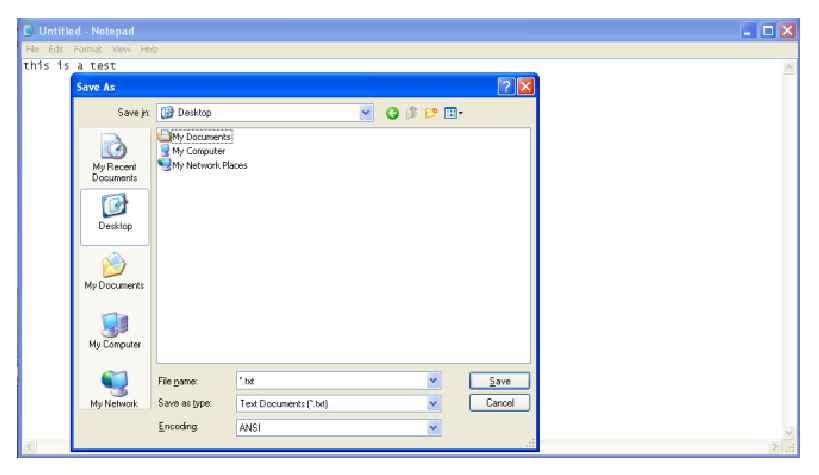
\includegraphics[width=65mm]{eps/figure17.eps}
\end{center}
\caption{Janela de Salvar Arquivo no Bloco de Notas.}\label{fig17}
\end{figure}

Abra o terminal do Python novamente e digite:

\begin{listing}
\begin{verbatim}
>>> f = open('c:\\teste.txt')
>>> print(f.read())
\end{verbatim}
\end{listing}

O conteúdo do arquivo que você acabou de criar será exibido.
\end{WINDOWS}

\begin{MAC}
Para ver como o \code{file} é usado, abra o Editor de Texto, clicando no ícone do editor (\includegraphics([width=12mm]{eps/textedit-icon.eps}). Digite algumas palavras e então salve o arquivo na Mesa, clicando em Arquivo e Salvar, com o nome `teste.txt'.

\begin{figure}
\begin{center}
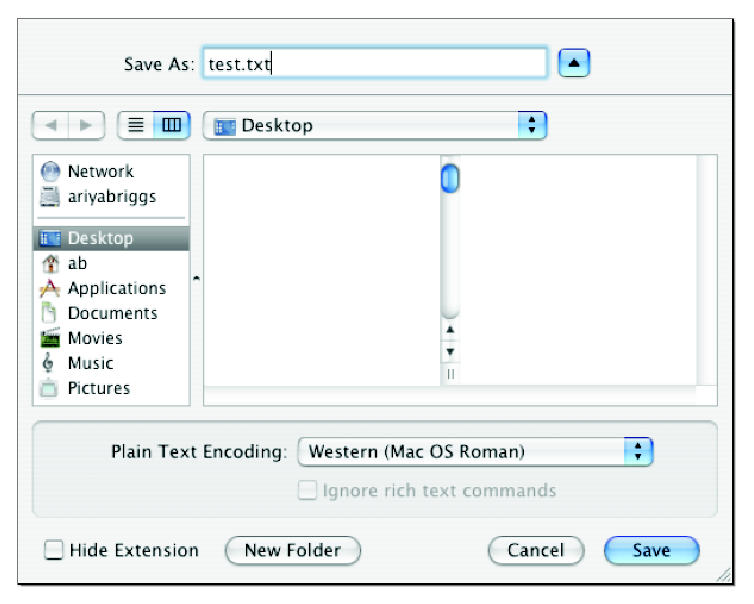
\includegraphics[width=65mm]{eps/figure18.eps}
\end{center}
\caption{Janela de Salvar Arquivo no Editor de Texto do Mac OS X.}\label{fig18}
\end{figure}

Abra o terminal do Python novamente e digite:

\begin{listing}
\begin{verbatim}
>>> f = open('Desktop/teste.txt')
>>> print(f.read())
\end{verbatim}
\end{listing}

O conteúdo do arquivo que você acabou de criar será exibido.
\end{MAC}

\begin{LINUX}
Para ver como o \code{file} é usado, abra um editor de texto, digite algumas palavras e então salve o arquivo no seu diretório `Home', clicando em Arquivo, Salvar e então selecionando o diretório `Home'. Digite o nome do arquivo `teste.txt` (veja na figura~\ref{fig19} por exemplo).

\begin{figure}
\begin{center}
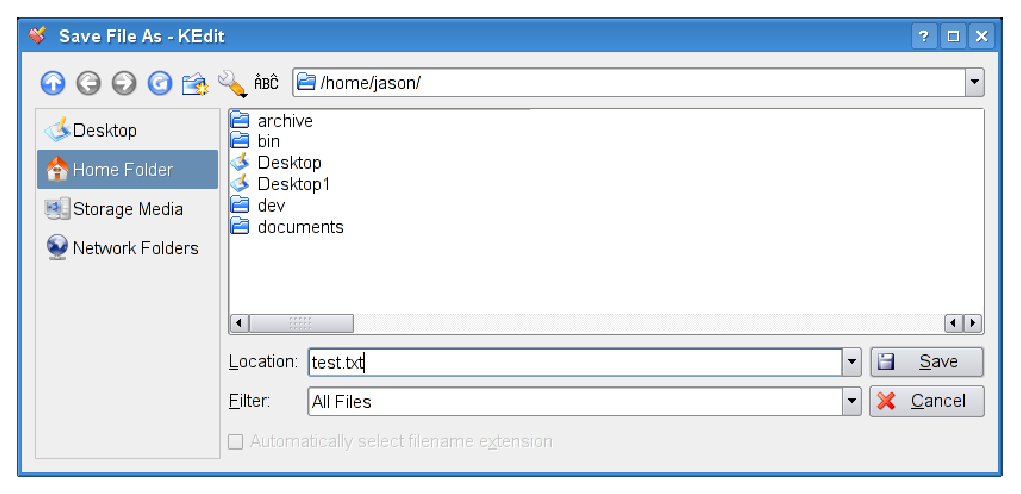
\includegraphics[width=65mm]{eps/figure19.eps}
\end{center}
\caption{Janela de Salvar Arquivo do Editor de Texto KEdit.}\label{fig19}
\end{figure}

Abra o terminal do Python novamente e digite:

\begin{listing}
\begin{verbatim}
>>> f = open('~/teste.txt')
>>> print(f.read())
\end{verbatim}
\end{listing}

\end{LINUX}

Então, o que esse pequeno trecho de código faz? A primeira linha chama a função \code{file}, passando o caminho do arquivo que você criou, como parâmetro. A função retorna um tipo de valor especial (chamado objeto) que representa um arquivo. Não é o arquivo em si; mas sim como se fosse um grande dedo apontando para o arquivo, dizendo ``AQUI ESTÁ ELE!!!'' O objeto de arquivo é armazenado na variável \code{f}.
\par
A próxima linha, chama uma função especial (\code{read}) no objeto de arquivo, para ler o seu conteúdo e imprimir o resultado no terminal. Por a variável \code{f} conter um objeto, isso significa que nós precisamos chamar a função `read' usando o símbolo ponto (.).

\fbox{\colorbox{PaleBlue}{\parbox{.75\linewidth} {
\par
O apêndice~\ref{app:builtinfunctions} (no final do livro) tem mais informações sobre as funções embutidas no Python.
\par
}}}

\section{Modules}\index{modules}

We've actually seen a couple of different ways to reuse code already. One is a standard function, which we can create ourselves, or use the functions built into Python (like \code{range} and \code{file} and \code{int} and \code{str}). Another is a special kind of function on objects---which we can call using the dot symbol---and the next are modules; which are a way of grouping lots of functions and objects together in useful ways. An example of this is the module `time'\index{modules!time}:

\begin{listing}
\begin{verbatim}
>>> import time
\end{verbatim}
\end{listing}

The import command is used to tell Python we want to access a module.  In the above example, we're saying we want to use the `time' module. We can then call functions and objects that are available in this module, using the dot symbol yet again:

\begin{listingignore}
\begin{verbatim}
>>> print(time.localtime())
(2006, 11, 10, 23, 49, 1, 4, 314, 1)
\end{verbatim}
\end{listingignore}

localtime\index{modules!time!localtime} is a function \emph{inside} the module time, that returns the current date and time, broken up into individual parts---year, month, day, hour, minute, second, day of the week, day of the year, and whether or not it's daylight savings (1 if it is, 0 if it isn't).  The individual parts are stored in a tuple (see \emph{Tuples and Lists} on page~\pageref{tuplesandlists}.  You can use another function in the time module to convert the datetime returned by localtime, into something a bit more understandable:

\begin{listingignore}
\begin{verbatim}
>>> t = time.localtime()
>>> print(time.asctime(t))
Sat Nov 18 22:37:15 2006
\end{verbatim}
\end{listingignore}

\noindent
We can do that all in a single line if we wanted to:

\begin{listingignore}
\begin{verbatim}
>>> print(time.asctime(time.localtime()))
Sat Nov 18 22:37:15 2006
\end{verbatim}
\end{listingignore}

Suppose you want to ask for someone to enter a value. You can do this using a \code{print} statement and the module `\code{sys}'\index{modules!sys}---imported the same way we imported the \code{time} module:

\begin{listing}
\begin{verbatim}
import sys
\end{verbatim}
\end{listing}

Inside the sys module is an object called `stdin'\index{modules!sys!stdin} (short for standard input).  stdin has a rather useful method (or function) called \code{readline}---which is used to read a line of text someone types on the keyboard (up until the point when they press the Enter key).  You can test \code{readline}, by entering the following command in the Python console:

\begin{listing}
\begin{verbatim}
>>> print(sys.stdin.readline())
\end{verbatim}
\end{listing}

If you then type some words, and press the Enter key, what you've typed will be printed to the console. Think back, for a moment, to the code we wrote earlier, using an if-statement:

\begin{listing}
\begin{verbatim}
if age >= 10 and age <= 13:
    print('you are %s' % age)
else:
    print('huh?')
\end{verbatim}
\end{listing}

Rather than creating the variable \code{age} beforehand, we can now ask someone to enter the value instead.  How about first turning the code into a function$\ldots$

\begin{listing}
\begin{verbatim}
>>> def your_age(age):
...     if age >= 10 and age <= 13:
...         print('you are %s' % age)
...     else:
...         print('huh?')
... 
\end{verbatim}
\end{listing}

Which can be called, by passing a number as the parameter value.  We'll test that it works properly, first:

\begin{listing}
\begin{verbatim}
>>> your_age(9)
huh?
>>> your_age(10)
you are 10
\end{verbatim}
\end{listing}

Now we know there are no problems with our function, we can change the function to ask for a person's age instead:

\begin{listing}
\begin{verbatim}
>>> def your_age():
...     print('Please enter your age')
...     age = int(sys.stdin.readline())
...     if age >= 10 and age <= 13:
...         print('you are %s' % age)
...     else:
...         print('huh?')
... 
\end{verbatim}
\end{listing}

Because \code{readline()} returns what a person typed as text (in other words, a string), we need to use the function \code{int} to convert it to a number (this so it will work correctly in the if-statement---check \emph{What's the difference} on page~\pageref{whatsthedifference} for more information about this).  To try it for yourself, call the your\_age function without any parameters, then type some text when `Please enter your age' appears:

\begin{listingignore}
\begin{verbatim}
>>> your_age()
Please enter your age
10
you are 10
>>> your_age()
Please enter your age
15
huh?
\end{verbatim}
\end{listingignore}

\noindent
\emph{The important thing to note here is that even though you're typing in a number (in the above case 10 or 15), readline always returns a string.}

\fbox{\colorbox{PaleBlue}{\parbox{.75\linewidth} {
\code{sys} and \code{time} are just two of the many modules that are included with Python.  For more information on some (but not all) Python modules, see Appendix~\ref{app:afewpythonmodules}.
}}}

\section{Things to try}

\emph{In this chapter we saw how to do recycling in Python; through the use of functions and modules.  We saw a little bit about the `scope' of variable, how variables outside of functions can be `seen' inside, whereas variables inside cannot be seen outside, and learned how to create our own functions using \code{def}}

\subsection*{Exercise 1}
In exercise 2 in Chapter~\ref{ch:againandagain}, we created a for-loop to work out the interest we might earn from \$100 over a period of 10 years.  That for-loop could easily be turned into a function.  Try creating a function which takes a starting amount, and a rate of interest.  You could call the function using code like:

\begin{listing}
\begin{verbatim}
calculate_interest(100, 0.03)
\end{verbatim}
\end{listing}

\subsection*{Exercise 2}
Take the function you've just created, and make it calculate interest for different periods---such as 5 years or 15 years.  Perhaps you could call it using code like:

\begin{listing}
\begin{verbatim}
calculate_interest(100, 0.03, 5)
\end{verbatim}
\end{listing}

\subsection*{Exercise 3}
Perhaps rather than a simple function, where we pass in the values as parameters, we can make a mini-program which asks someone for the values (using the \code{sys.stdin.readline()} function).  In this case, we'll call the function without any parameters at all:

\begin{listing}
\begin{verbatim}
calculate_interest()
\end{verbatim}
\end{listing}

\noindent
To create this mini-program requires a function that we haven't talked about yet: \code{float}. The \code{float} function is a bit like the \code{int} function, except it converts strings into what is called floating point numbers (which we discussed briefly in Chapter~\ref{ch:8multipliedby3.57}).  Floating point numbers are numbers with a decimal place (.), such as 20.3 or 2541.933.

\newpage
